\section{Execution-Time Semantics and Corporate Actions}
\label{app:timing}
\setcounter{equation}{0}
\subsection{Three timestamps per observation}
An observation has a decision date, an entry date, and an exit date. Treating these as interchangeable is a common source of hidden look-ahead. For a feature row indexed by session $t$, the decision occurs after close $t$, entry occurs at open $t+1$, and the outcome is known at open $t+2$. The model uses the signal-date index to retrieve features, the exit date to determine training eligibility, and entry/exit dates to assign holding returns to a reporting period. None of these operations can be replaced safely by assuming that an earlier row index implies an already realized outcome.

Table~\ref{tab:trace} gives the first six actual holdout observations. The first signal is formed on 31 December 2021 even though the first investment interval belongs wholly to 2022. On 3 January 2022, the model can be refitted using a label that ends at that morning's opening, but not using the label associated with the immediately preceding decision if it ends on 4 January. The code stores the maximum label exit in every fit audit so this distinction can be checked directly.

\begin{table}[htbp]
 \centering\small
 \caption{Actual beginning-of-holdout trace. Forecasts and realized holding returns are in basis points. These are recorded outcomes, not a synthetic execution example.}
 \label{tab:trace}
 \begin{tabular}{lllrrr}
\toprule
Decision & Entry & Exit & Forecast (bps) & Realized (bps) & $w$ \\
\midrule
2021-12-31 & 2022-01-03 & 2022-01-04 & 4.832 & 61.306 & 1 \\
2022-01-03 & 2022-01-04 & 2022-01-05 & 12.675 & -42.986 & 1 \\
2022-01-04 & 2022-01-05 & 2022-01-06 & 12.396 & -194.274 & 1 \\
2022-01-05 & 2022-01-06 & 2022-01-07 & 18.088 & 1.282 & 1 \\
2022-01-06 & 2022-01-07 & 2022-01-10 & 21.408 & -112.191 & 1 \\
2022-01-07 & 2022-01-10 & 2022-01-11 & 15.164 & 54.679 & 1 \\
\bottomrule
\end{tabular}

\end{table}

The action chosen at the close is a target for the following opening auction. Until that opening, the previous position continues to bear the market movement of its own interval. At the next open the previous interval is marked, any new target is executed, and the next interval begins. This chronological decomposition ensures that the opening gap preceding entry is not credited to a position chosen only after the prior close. It also ensures that selling fees are assigned when the position changes, rather than appended to an unrelated later return.

\subsection{Dividend entitlement and the target formula}
Suppose a share is purchased at $O_{t+1}$. At exit its economic value consists of the sale price $O_{t+2}$ and, if the exit is an ex-dividend date, the entitled distribution receivable $D_{t+2}$. The resulting gross wealth factor is
\begin{equation}
 1+y_t=\frac{O_{t+2}+D_{t+2}}{O_{t+1}}.
 \label{eq:app-dividend}
\end{equation}
If $t+1$ itself is an ex-date, a purchase at that open does not receive $D_{t+1}$. Adding that amount to the numerator would overstate performance. Conversely, omitting $D_{t+2}$ when the position was carried into that ex-date would understate it. A unit test places a synthetic dividend on a known session and checks both cases independently.

This treatment is an ex-date total-return convention. It treats the receivable as reinvestable at the exit open; the actual payment date is not modeled. Across consecutive invested intervals, the convention compounds the dividend into portfolio wealth. A real account might instead carry a receivable or temporarily hold cash until payment. The convention is applied consistently to Ridge, MA20, and buy-and-hold, and is disclosed because internal consistency does not remove its economic approximation.

\subsection{Raw opens and adjusted feature prices}
The data source supplies OHLC and a separate adjusted close. Execution uses OHLC with explicit distributions, while features use trailing adjusted-price ratios. The absence of splits in this SPY interval means no split-share conversion is needed in the implemented P\&L. The code refuses a split rather than assuming that vendor field semantics automatically solve every share-accounting problem. A different asset or extended sample containing splits would require an additional implementation and verification step before this target could be reused.

Vendor adjusted-close returns need not equal explicit cash-dividend returns at machine precision. For close $C_t$, define the explicit series
\begin{equation}
 r_t^{\mathrm{cash}}=\frac{C_t+D_t}{C_{t-1}}-1,
 \qquad r_t^{\mathrm{vendor}}=\frac{A_t}{A_{t-1}}-1.
\end{equation}
Their mean absolute difference in this snapshot is 0.00594 bps and their maximum absolute difference is 2.52010 bps. These differences reflect adjustment/reinvestment conventions and numerical representation. We report them rather than asserting exact equivalence. They do not enter execution twice: the portfolio return always follows Eq.~\eqref{eq:app-dividend}.

\begin{table}[htbp]
 \centering\small
 \caption{Representative dividend checks from the first and last events in the snapshot. $\Delta$ is vendor return minus explicit cash return. No representative split check is applicable because no split occurs.}
 \label{tab:events}
 \begin{tabular}{lrrrr}
\toprule
Ex-date & Dividend (USD) & Vendor return (\%) & Cash return (\%) & $\Delta$ (bps) \\
\midrule
2010-03-19 & 0.4800 & -0.50618 & -0.50410 & -0.20801 \\
2010-06-18 & 0.5310 & 0.10842 & 0.10790 & 0.05112 \\
2025-09-19 & 1.8310 & 0.49528 & 0.49392 & 0.13685 \\
2025-12-19 & 1.9930 & 0.90636 & 0.90367 & 0.26878 \\
\bottomrule
\end{tabular}

\end{table}

\subsection{Calendar completeness and outliers}
The observed 4,024 dates equal the expected XNYS session set over the observed endpoints. The check uses set differences in both directions, so a duplicate or accidental non-trading-day observation cannot cancel a missing session by preserving the row count. Special exchange closures are included in the calendar; the five-calendar-day gap ending 31 October 2012 therefore does not imply a missing trading observation. Half-days remain trading sessions and contribute one opening-to-opening interval when adjacent data are available.

Finite-price and OHLC ordering checks are separate from calendar verification. A complete calendar does not guarantee valid prices, and valid prices do not guarantee complete dates. Missing values cause failure rather than forward filling. Extreme observed returns are preserved because discarding crises after looking at the full history can alter the target distribution. No robust-scaling or clipping parameter is estimated from the full sample.

\section{Feature Invariance, Scaling, and Eligible Training Sets}
\label{app:features}
\subsection{Why trailing ratios do not use an absolute adjusted level}
Future corporate actions can rescale earlier vendor-adjusted prices. The relevant question is whether that rescaling changes the information used by an earlier predictor, not whether the downloaded file was created at the historical decision time. For the particular features used here, a common factor across the required lookback cancels algebraically.

\begin{proposition}[Common-factor invariance]
\label{prop:invariance}
Fix a decision session $t$. Suppose an adjustment replaces $A_s$ by $\widetilde A_s=\lambda A_s$ for all $s\in\{t-20,\ldots,t\}$, where $\lambda>0$. The five-dimensional feature vector defined in Eqs.~\eqref{eq:mom}--\eqref{eq:vol} is unchanged.
\end{proposition}
\begin{proof}
For each $k\in\{1,5,20\}$,
\begin{equation}
 \frac{\widetilde A_t}{\widetilde A_{t-k}}-1
 =\frac{\lambda A_t}{\lambda A_{t-k}}-1
 =\frac{A_t}{A_{t-k}}-1.
\end{equation}
Similarly, the denominator of the moving-average ratio is multiplied by $\lambda$, so $\widetilde g_t=g_t$. Every one-session return needed for $v_t$ has numerator and denominator in the stated window; each ratio is unchanged. The vector of 20 returns, its sample mean, and its sample standard deviation are therefore unchanged.\qedhere
\end{proof}

The proposition is deliberately narrow. It does not cover arbitrary data corrections, changing field definitions, or a transformation that is nonconstant within the relevant earlier lookback. Nor does it license future corporate-action quantities as independent predictive inputs. The source snapshot and digest remain necessary. A regression test multiplies all adjusted closes through a cutoff by a common factor and checks equality of all earlier features up to numerical tolerance.

\subsection{Exact lookbacks and missing-value policy}
The 20-session return uses $A_t$ and $A_{t-20}$. The moving average uses 20 levels from $A_{t-19}$ through $A_t$. Volatility uses the 20 returns ending on those dates and consequently also requires $A_{t-20}$. All five features become simultaneously available after 20 warm-up sessions. Using a partial initial rolling window would create a different feature definition and is not allowed silently.

The raw-history range extends beyond the first possible trading observation for this reason. The full history contains 4,024 sessions; deleting 20 warm-up rows and two terminal unknown labels leaves 4,002 complete samples. Validation and testing select their periods from that common sample using holding dates. Other missing data would require inspection and a documented source correction, not automatic interpolation that might use later information.

\subsection{Training-only standardization}
At refit $d$, for feature coordinate $j$ and $n_d=|\mathcal T_d|$,
\begin{align}
 \mu_{d,j}&=\frac{1}{n_d}\sum_{t\in\mathcal T_d}x_{t,j},\\
 s_{d,j}^2&=\frac{1}{n_d}\sum_{t\in\mathcal T_d}
 (x_{t,j}-\mu_{d,j})^2.
 \label{eq:scaler}
\end{align}
This denominator is $n_d$, matching \code{StandardScaler}; it differs from the denominator 19 used to define the 20-return volatility feature. Confusing the two standard deviations would not be a timing leak, but would change the numerical penalty interpretation and prevent exact reconstruction. The scaler is fitted with the model on the same eligible rows and then remains fixed until the next refit.

\begin{table}[htbp]
 \centering\small
 \caption{Recorded training means and scales at the first and last holdout fits. Values use decimal-return units, not percentage points. These differ across windows and are not estimated from a full-sample fit.}
 \label{tab:scaler}
 \begin{tabular}{lrrrr}
\toprule
Feature & First mean & First scale & Last mean & Last scale \\
\midrule
\texttt{return\_1} & 0.000734 & 0.011871 & 0.000623 & 0.010769 \\
\texttt{return\_5} & 0.003582 & 0.023666 & 0.002992 & 0.022403 \\
\texttt{return\_20} & 0.014244 & 0.046303 & 0.012595 & 0.041769 \\
\texttt{ma\_gap\_20} & 0.006368 & 0.026229 & 0.005504 & 0.023464 \\
\texttt{volatility\_20} & 0.009079 & 0.007716 & 0.009757 & 0.004768 \\
\bottomrule
\end{tabular}

\end{table}

\subsection{Observable labels and scheduled updating}
For a decision close $d$, define $\mathcal E_d=\{t:t<d,\ e(t)\le d\}$. The implemented training set is its latest 1,260 rows. Because each included outcome ends at or before open $d$, and all its features are available by close $t<d$, the entire training pair is observable by close $d$. Outcomes ending later than $d$ are excluded even if the feature row is already known. The filter is equivalent to the appropriate non-overlap rule for this one-interval target; an arbitrary additional embargo is not needed to make already mature, non-overlapping labels observable.

This reasoning would change for a longer holding horizon, delayed fundamental announcements, revised macroeconomic vintages, or overlapping labels used in validation. In those settings, timestamping a row by calendar date would not establish its publication time, and a revised maturity or purging rule would be required. The current project avoids those extra information sources rather than claiming a general solution to every financial-data timing problem.

Monthly refitting updates model parameters under a fixed policy. There is no requirement that all training samples precede the beginning of the entire holdout: once an earlier test outcome occurs, it becomes legitimate past information for a later decision. What remains locked is the procedure that maps available data to predictions, including features, window, refit schedule, penalty, and position rule. Reselecting these choices using holdout outcomes would be a separate and invalid use of the final evaluation.

\subsection{Objective scaling and coefficient interpretation}
For centered standardized features $Z$ and centered outcomes $y$, Ridge has the solution
\begin{equation}
 \widehat\beta=(Z^{\mathsf T}Z+\alpha I)^{-1}Z^{\mathsf T}y,
 \label{eq:ridge-solution}
\end{equation}
under the stated sum-loss convention. The implementation uses SVD rather than explicitly forming the inverse. With standardized features, coefficients represent decimal-return changes for a one-training-SD feature change. Multiplying a coefficient by $10^4$ expresses that conditional association in basis points. It is not an elasticity and not the effect of a one-percentage-point raw feature change.

The penalty reduces sensitivity to near-collinearity, but a ridge coefficient may still change sign as the window changes. The five technical signals share price history and overlap in their lookbacks. A sign on one coordinate is conditional on the others and cannot be interpreted independently as evidence for a structural momentum or reversal mechanism. Appendix~\ref{app:fits} retains both paths and descriptive summaries without using them to prune the specification.

\section{Portfolio Accounting and Cost Attribution}
\label{app:accounting}
\subsection{From decisions to a self-consistent interval path}
For each interval $i$, the portfolio first moves from the previous target $w_{i-1}$ to the new target $w_i$ at the entry open. Its fee is a fraction $cq_i$ of pre-trade wealth, where $q_i=|w_i-w_{i-1}|$. The remaining wealth then earns $w_i y_i$, with the uninvested part earning zero. At the final exit, an invested portfolio liquidates and pays the additional cost. The interval and terminal factors are
\begin{align}
 G_i(c)&=(1-cq_i)(1+w_i y_i),\label{eq:appgrowth}\\
 V_N(c)&=\left[\prod_{i=1}^N G_i(c)\right](1-cw_N).
 \label{eq:terminal}
\end{align}
The assumption is a pre-trade-equity haircut. If a broker charges a fee on purchased notional while imposing exact full-investment constraints, the share quantity can require a slightly different cash equation. Equation~\eqref{eq:appgrowth} is therefore an explicit research convention. It is not silently described as a detailed brokerage implementation. All strategies share the convention.

Binary weights simplify the bookkeeping. An unchanged fully invested portfolio remains fully invested after its asset return; an unchanged cash portfolio remains cash. There is no fractional target drift to rebalance. Dividends are incorporated by the declared total-return convention. A continuously rebalanced fractional-weight benchmark would need its own cash and turnover treatment; it cannot be produced by simply copying this binary-trade count.

\subsection{Proof and interpretation of the exact drag identity}
\begin{proof}[Proof of Proposition~\ref{prop:drag}]
For fixed positions and returns, every market-return factor $(1+w_i y_i)$ appears in both $V_N(c)$ and $V_N(0)$ and cancels. Since $w_i\in\{0,1\}$, each $q_i$ is also zero or one, and $(1-cq_i)=(1-c)^{q_i}$. The terminal factor is $(1-c)^{w_N}$. Hence
\begin{align}
 \frac{V_N(c)}{V_N(0)}
 &=\left[\prod_{i=1}^N(1-c)^{q_i}\right](1-c)^{w_N}\\
 &=(1-c)^{\sum_iq_i+w_N}=(1-c)^K.
\end{align}
All factors are positive under the proposition's conditions, so the ratio is well defined.\qedhere
\end{proof}

Taking logarithms gives an exact annualized log-wealth drag,
\begin{equation}
 L(c)=-\frac{252}{N}\log\frac{V_N(c)}{V_N(0)}
 =-\frac{252K}{N}\log(1-c).
 \label{eq:logdrag}
\end{equation}
For small $c$, $-\log(1-c)\approx c$, producing the intuitive first-order relationship $L(c)\approx252Kc/N$. The numerical comparison in Table~\ref{tab:drag} uses the exact formula, not the approximation. The builder checks the identity against the saved net and gross terminal wealth values before emitting the table.

\begin{table}[htbp]
 \centering\small
 \caption{Exact fee attribution at 5 bps, conditional on the same frozen positions. Annual log drag differs from a difference in arithmetic returns or percentage-point CAGR.}
 \label{tab:drag}
 \begin{tabular}{lrrr}
\toprule
Strategy & $K$ & Net/gross wealth & Annual log drag (\%) \\
\midrule
Ridge & 246 & 0.884236 & 3.094 \\
MA20 & 102 & 0.950267 & 1.283 \\
Buy-and-hold & 2 & 0.999000 & 0.025 \\
\bottomrule
\end{tabular}

\end{table}

The identity shows how much wealth is removed by the declared fees, but does not by itself explain why the gross strategy differs from buy-and-hold. That difference reflects which returns are held and which are missed. It also does not identify a counterfactual strategy that would trade less: changing the threshold would change $w_i$, the gross market factors, and $K$ together. Reporting a lower-cost threshold without a separate evaluation would mix accounting attribution with post-hoc strategy selection.

\subsection{A small synthetic accounting example}
Consider three hypothetical holding returns $(0.01,-0.02,0.03)$ and target weights $(1,0,1)$. These numbers illustrate the formula only and do not replace any empirical return. Beginning from cash, entry/switch turnover is $(1,1,1)$, and final liquidation adds one more unit. With cost $c$, terminal wealth is
\begin{equation}
 V_3(c)=[(1-c)1.01]\,[(1-c)]\,[(1-c)1.03]\,(1-c)
 =(1-c)^4(1.01)(1.03).
\end{equation}
The negative middle asset return is not earned because the portfolio is in cash, but the sale into cash still incurs a fee. An always-cash path earns one with no fees; an always-invested path incurs exactly two fee units, at entry and exit. The integrity suite checks all three cases. Charging fees only on purchases, omitting final liquidation, or charging a daily fee on unchanged positions would produce a different and incorrect implementation of the declared rule.

\subsection{Metric definitions and calendar aggregation}
Initial capital is one. Terminal wealth determines total return and CAGR. Annualized arithmetic return and volatility use 252 intervals and sample standard deviation; Sharpe divides those quantities with a zero reference rate. Maximum drawdown is
\begin{equation}
 \mathrm{MDD}=\min_i\left(\frac{V_i}{\max(1,V_1,\ldots,V_i)}-1\right).
\end{equation}
Including initial capital is necessary: otherwise a loss in the first interval would be excluded from the drawdown history. The implementation has a dedicated regression test for this case.

Calendar-year returns compound only that year's continuous-path net interval returns. Costs are not reset on 1 January. The initial fee belongs to the first interval and final liquidation belongs to the last interval; intervening year boundaries create no trades. Annual sample counts differ because market calendars differ. Annual returns in the supplement are realized compounded returns, while an annual row's CAGR may use $252/N_{\mathrm{year}}$ and therefore differ slightly. The main annual table intentionally uses realized return rather than relabeling it as a full-period CAGR.

\section{Complete Empirical Results and Frozen-Path Diagnostics}
\label{app:empirical}
\subsection{Complete validation search}
Table~\ref{tab:validationfull} includes all four candidates, not only the selected row. The selection criterion is net Sharpe at 5 bps. The forecast $R^2$ columns are descriptive and are not a second objective used to resolve the selected outcome. Penalties 0.1 and 1 have identical validation trading results but different forecast errors because the binary position map can hide changes in magnitude that do not cross zero.

\begin{table}[htbp]
 \centering\small
 \caption{Full pre-declared validation grid. CAGR, volatility, and drawdown are in percent; turnover is the total charged one-way amount. Validation contains 756 holding intervals per candidate.}
 \label{tab:validationfull}
 \begin{tabular}{lrrrrrr}
\toprule
$\alpha$ & CAGR (\%) & Sharpe & Vol. (\%) & MDD (\%) & Turnover & $R^2_{\mathrm{OOS}}$ \\
\midrule
0.1 & 22.33 & 1.2060 & 18.08 & -32.05 & 136 & -0.01442 \\
1 & 22.33 & 1.2060 & 18.08 & -32.05 & 136 & -0.01434 \\
10 & 19.15 & 1.0767 & 17.76 & -32.05 & 134 & -0.01364 \\
100 & 18.64 & 1.0310 & 18.21 & -32.05 & 116 & -0.01089 \\
\bottomrule
\end{tabular}

\end{table}

\begin{figure}[htbp]
 \centering
 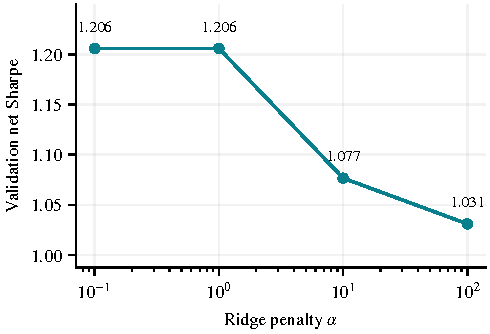
\includegraphics[width=.56\textwidth]{generated/validation.pdf}
 \caption{Validation penalty path. Only these four settings are compared. There is no corresponding holdout penalty curve because the final period is reserved for the selected setting.}
 \label{fig:valappendix}
\end{figure}

Validation returns are not independent observations from the final test, and overlapping rolling training windows create dependence among successive forecasts. The selected validation Sharpe is consequently a development statistic, not a clean estimate of deployable performance. The experiment does not interpret the gap between validation and testing as a uniquely identified structural break. Multiple explanations, including sampling noise and selection optimism, remain consistent with the evidence.

\subsection{All cost scenarios and annual outcomes}
Table~\ref{tab:costfull} reports all three strategies at zero, five, and ten basis points. Positions and predictions are fixed across scenarios. The passive benchmark's near-flat cost curve reflects its two charged trades; MA20's intermediate sensitivity reflects its 102 trades; Ridge is most sensitive with 246. These comparisons would be obscured if costs were waived for one strategy or if each scenario were allowed to reselect a different model.

\begin{table}[htbp]
 \centering\small
 \caption{Full cost sensitivity of the same frozen holding paths. Final wealth includes liquidation. Cost values are assumptions rather than estimates of actual opening-auction spreads or impact.}
 \label{tab:costfull}
 \begin{tabular}{llrrrr}
\toprule
Strategy & bps & CAGR (\%) & Sharpe & MDD (\%) & Final wealth \\
\midrule
Ridge & 0 & 9.88 & 0.678 & -20.97 & 1.4546 \\
MA20 & 0 & 5.03 & 0.508 & -17.84 & 1.2156 \\
Buy-and-hold & 0 & 11.20 & 0.672 & -26.28 & 1.5254 \\
Ridge & 5 & 6.54 & 0.481 & -22.20 & 1.2863 \\
MA20 & 5 & 3.69 & 0.389 & -19.14 & 1.1552 \\
Buy-and-hold & 5 & 11.18 & 0.670 & -26.28 & 1.5238 \\
Ridge & 10 & 3.29 & 0.284 & -23.89 & 1.1373 \\
MA20 & 10 & 2.37 & 0.271 & -20.43 & 1.0977 \\
Buy-and-hold & 10 & 11.15 & 0.669 & -26.28 & 1.5223 \\
\bottomrule
\end{tabular}

\end{table}

\begin{table}[htbp]
 \centering\small
 \caption{Full calendar-year net results at 5 bps. Return, volatility, and exposure are in percent. Turnover is assigned to the intervals where the continuous portfolio actually trades.}
 \label{tab:annualfull}
 \begin{tabular}{llrrrrr}
\toprule
Strategy & Year & Return (\%) & Vol. (\%) & Sharpe & Exposure (\%) & Turnover \\
\midrule
Ridge & 2022 & -13.80 & 20.11 & -0.644 & 65.60 & 60 \\
Ridge & 2023 & 16.15 & 10.60 & 1.478 & 67.20 & 69 \\
Ridge & 2024 & 16.90 & 9.47 & 1.696 & 73.02 & 59 \\
Ridge & 2025 & 9.88 & 19.59 & 0.582 & 71.60 & 58 \\
MA20 & 2022 & -17.99 & 13.28 & -1.439 & 42.00 & 32 \\
MA20 & 2023 & 19.93 & 9.61 & 1.954 & 67.20 & 21 \\
MA20 & 2024 & 9.09 & 9.18 & 0.993 & 80.16 & 23 \\
MA20 & 2025 & 7.67 & 10.69 & 0.751 & 71.60 & 26 \\
Buy-and-hold & 2022 & -18.82 & 24.15 & -0.750 & 100.00 & 1 \\
Buy-and-hold & 2023 & 27.09 & 13.47 & 1.861 & 100.00 & 0 \\
Buy-and-hold & 2024 & 25.40 & 12.65 & 1.854 & 100.00 & 0 \\
Buy-and-hold & 2025 & 17.79 & 20.41 & 0.910 & 100.00 & 1 \\
\bottomrule
\end{tabular}

\end{table}

The annual table emphasizes that a lower full-period maximum drawdown need not mean consistently better returns. Ridge loses less than buy-and-hold in 2022, but its realized return is lower in the following three years. A rule that alternated between these strategies after seeing the annual table would be a new, hindsight-based portfolio rather than the evaluated experiment. No such switching rule is included.

\begin{figure}[htbp]
 \centering
 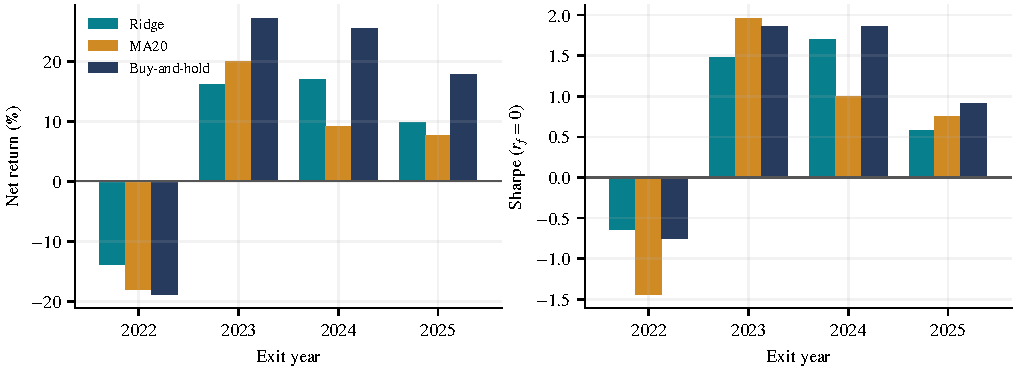
\includegraphics[width=.94\textwidth]{generated/annual.pdf}
 \caption{Annual net return and Sharpe. These panels describe the four observed years; they do not provide four independent replications of a strategy-selection experiment.}
 \label{fig:annualappendix}
\end{figure}

\subsection{Forecast distribution and direction classification}
Forecast MSE is 0.0001336494, compared with 0.0001329298 for the past-only historical mean. Their ratio yields $R^2_{\mathrm{OOS}}=\OOSRsquared{}$. All errors refer to the executable label, not a more convenient close-to-close target. Table~\ref{tab:distribution} reports the scale of forecasts and outcomes in basis points; the forecast distribution is much narrower than the realized-return distribution.

\begin{table}[htbp]
 \centering\small
 \caption{Descriptive distribution of the frozen holdout forecasts and outcomes. SD is the sample standard deviation. These statistics are not used for full-sample scaling or threshold selection.}
 \label{tab:distribution}
 \begin{tabular}{lrrrrr}
\toprule
Series (bps) & Mean & SD & Min. & Median & Max. \\
\midrule
Model forecast & 5.867 & 12.797 & -46.704 & 4.091 & 73.544 \\
Realized holding return & 4.879 & 115.328 & -658.430 & 8.726 & 784.897 \\
Historical-mean forecast & 5.852 & 0.842 & 4.271 & 6.160 & 7.590 \\
\bottomrule
\end{tabular}

\end{table}

\begin{figure}[htbp]
 \centering
 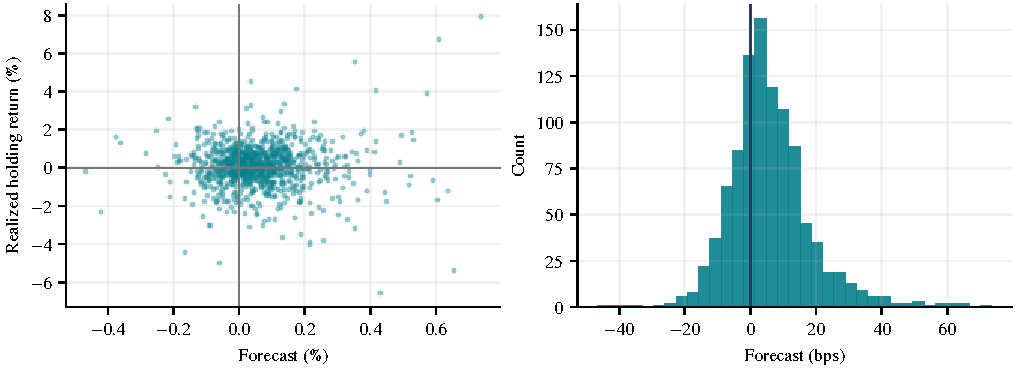
\includegraphics[width=.94\textwidth]{generated/predictions.pdf}
 \caption{Frozen forecasts against realized returns, and the distribution of forecast scores. The zero line is the pre-specified investment threshold, not a threshold fitted to this plot.}
 \label{fig:predictionappendix}
\end{figure}

\begin{table}[htbp]
 \centering\small
 \caption{Direction classification and position map. Positive forecasts imply SPY; all other forecasts imply cash. Counts use the realized asset return sign, not the portfolio return after costs.}
 \label{tab:confusion}
 \begin{tabular}{lrrr}
\toprule
Forecast position & $y>0$ & $y\leq 0$ & Total \\
\midrule
SPY & 371 & 324 & 695 \\
Cash & 165 & 142 & 307 \\
\bottomrule
\end{tabular}

\end{table}

The confusion matrix makes clear why a hit rate is not an economic objective. A correct decision on a tiny return counts as much as a correct decision on a large return. Predicting positive returns frequently may also achieve a favorable hit rate simply when the unconditional positive-return fraction is high. The matrix is therefore interpreted alongside magnitude, exposure, turnover, and net wealth. It is not used to recalibrate a probability threshold or to claim a classification advantage.

\begin{table}[htbp]
 \centering\small
 \caption{Underlying realized holding returns conditional on Ridge's frozen position. The cash row reports returns that were not earned; it does not assume a hypothetical cash strategy earns those asset returns.}
 \label{tab:conditional}
 \begin{tabular}{lrrrr}
\toprule
Ridge decision & Count & Mean $y$ (bps) & SD (bps) & Positive (\%) \\
\midrule
Invested intervals & 695 & 6.097 & 118.821 & 53.38 \\
Cash intervals & 307 & 2.121 & 107.137 & 53.75 \\
\bottomrule
\end{tabular}

\end{table}

Conditional returns are a descriptive partition of the single test path. They are neither randomized treatment effects nor independent samples, and differences can be affected by the dates at which the model is invested. We do not turn this partition into an additional significance claim. Its purpose is to connect the model's action to the asset returns that were held or missed, while keeping fees in the separate portfolio accounting.

\subsection{Exposure and the ex post diagnostic}
Figure~\ref{fig:exposureappendix} shows monthly mean exposure. These averages are summaries of binary daily positions, not fractional weights used in execution. The ex post constant-exposure diagnostic multiplies the underlying holding return by the realized average Ridge exposure, approximately 0.6936, and ignores fractional rebalancing costs. It has gross CAGR 8.03\%, volatility 12.70\%, and Sharpe 0.672 in this path. These values are not included in the investable benchmark table because the exposure was learned from the holdout.

\begin{figure}[htbp]
 \centering
 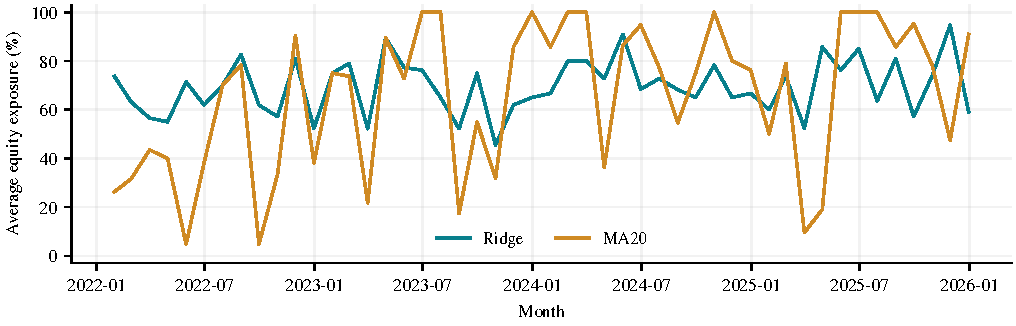
\includegraphics[width=.94\textwidth]{generated/exposure.pdf}
 \caption{Monthly average equity exposure. Time in cash reduces participation in both losses and gains. The visual pattern is a diagnostic of the frozen decision rule, not an additional market-state model.}
 \label{fig:exposureappendix}
\end{figure}

An investable risk-matched comparison would choose its risk budget using information available before the evaluated interval. It would also specify how weights respond to changes in wealth and how rebalancing costs are charged. That construction is outside this minimal experiment. Keeping the current series labeled ex post prevents an appealing diagnostic from being misrepresented as a strategy that could have been selected in advance.

\FloatBarrier
\section{Monthly Fits and Parameter Audit}
\label{app:fits}
The final holdout contains 49 fits. The first occurs at the 31 December 2021 decision close; the first decision in January creates the next scheduled fit, followed by each subsequent month through December 2025. Every fit has 1,260 training observations. The complete boundaries are retained in Table~\ref{tab:fitaudit}. The latest label exit never exceeds the fit date. The last training signal can be earlier than the previous exchange session because of the two-session target offset.

The boundary table is a useful audit but does not, by itself, prove that every processing stage is past-only. For that reason it is supplemented by tests that compare actual scaler means with the eligible-window means and by future-perturbation tests that check predictions and audit records. The combination of an explicit timing rule, exported boundaries, and behavioral tests is stronger than relying on an assertion of rolling estimation alone.

\begin{table}[htbp]
 \centering\scriptsize
 \caption{All final-holdout fit boundaries. The latest label exit is already observed at the fit-date open. A fixed training sample count does not imply a fixed calendar span because exchange-session calendars differ across years.}
 \label{tab:fitaudit}
 \setlength{\tabcolsep}{9pt}
 \begin{tabular}{llllr}
\toprule
Fit date & First training signal & Last training signal & Latest label exit & $N$ \\
\midrule
2021-12-31 & 2016-12-28 & 2021-12-29 & 2021-12-31 & 1260 \\
2022-01-03 & 2016-12-29 & 2021-12-30 & 2022-01-03 & 1260 \\
2022-02-01 & 2017-01-30 & 2022-01-28 & 2022-02-01 & 1260 \\
2022-03-01 & 2017-02-27 & 2022-02-25 & 2022-03-01 & 1260 \\
2022-04-01 & 2017-03-30 & 2022-03-30 & 2022-04-01 & 1260 \\
2022-05-02 & 2017-04-28 & 2022-04-28 & 2022-05-02 & 1260 \\
2022-06-01 & 2017-05-30 & 2022-05-27 & 2022-06-01 & 1260 \\
2022-07-01 & 2017-06-28 & 2022-06-29 & 2022-07-01 & 1260 \\
2022-08-01 & 2017-07-27 & 2022-07-28 & 2022-08-01 & 1260 \\
2022-09-01 & 2017-08-29 & 2022-08-30 & 2022-09-01 & 1260 \\
2022-10-03 & 2017-09-28 & 2022-09-29 & 2022-10-03 & 1260 \\
2022-11-01 & 2017-10-27 & 2022-10-28 & 2022-11-01 & 1260 \\
2022-12-01 & 2017-11-28 & 2022-11-29 & 2022-12-01 & 1260 \\
2023-01-03 & 2017-12-28 & 2022-12-29 & 2023-01-03 & 1260 \\
2023-02-01 & 2018-01-29 & 2023-01-30 & 2023-02-01 & 1260 \\
2023-03-01 & 2018-02-26 & 2023-02-27 & 2023-03-01 & 1260 \\
2023-04-03 & 2018-03-29 & 2023-03-30 & 2023-04-03 & 1260 \\
2023-05-01 & 2018-04-26 & 2023-04-27 & 2023-05-01 & 1260 \\
2023-06-01 & 2018-05-29 & 2023-05-30 & 2023-06-01 & 1260 \\
2023-07-03 & 2018-06-27 & 2023-06-29 & 2023-07-03 & 1260 \\
2023-08-01 & 2018-07-26 & 2023-07-28 & 2023-08-01 & 1260 \\
2023-09-01 & 2018-08-28 & 2023-08-30 & 2023-09-01 & 1260 \\
2023-10-02 & 2018-09-26 & 2023-09-28 & 2023-10-02 & 1260 \\
2023-11-01 & 2018-10-26 & 2023-10-30 & 2023-11-01 & 1260 \\
2023-12-01 & 2018-11-27 & 2023-11-29 & 2023-12-01 & 1260 \\
2024-01-02 & 2018-12-27 & 2023-12-28 & 2024-01-02 & 1260 \\
2024-02-01 & 2019-01-29 & 2024-01-30 & 2024-02-01 & 1260 \\
2024-03-01 & 2019-02-27 & 2024-02-28 & 2024-03-01 & 1260 \\
2024-04-01 & 2019-03-27 & 2024-03-27 & 2024-04-01 & 1260 \\
2024-05-01 & 2019-04-29 & 2024-04-29 & 2024-05-01 & 1260 \\
2024-06-03 & 2019-05-30 & 2024-05-30 & 2024-06-03 & 1260 \\
2024-07-01 & 2019-06-26 & 2024-06-27 & 2024-07-01 & 1260 \\
2024-08-01 & 2019-07-29 & 2024-07-30 & 2024-08-01 & 1260 \\
2024-09-03 & 2019-08-28 & 2024-08-29 & 2024-09-03 & 1260 \\
2024-10-01 & 2019-09-26 & 2024-09-27 & 2024-10-01 & 1260 \\
2024-11-01 & 2019-10-29 & 2024-10-30 & 2024-11-01 & 1260 \\
2024-12-02 & 2019-11-26 & 2024-11-27 & 2024-12-02 & 1260 \\
2025-01-02 & 2019-12-27 & 2024-12-30 & 2025-01-02 & 1260 \\
2025-02-03 & 2020-01-28 & 2025-01-30 & 2025-02-03 & 1260 \\
2025-03-03 & 2020-02-25 & 2025-02-27 & 2025-03-03 & 1260 \\
2025-04-01 & 2020-03-25 & 2025-03-28 & 2025-04-01 & 1260 \\
2025-05-01 & 2020-04-24 & 2025-04-29 & 2025-05-01 & 1260 \\
2025-06-02 & 2020-05-26 & 2025-05-29 & 2025-06-02 & 1260 \\
2025-07-01 & 2020-06-23 & 2025-06-27 & 2025-07-01 & 1260 \\
2025-08-01 & 2020-07-24 & 2025-07-30 & 2025-08-01 & 1260 \\
2025-09-02 & 2020-08-24 & 2025-08-28 & 2025-09-02 & 1260 \\
2025-10-01 & 2020-09-23 & 2025-09-29 & 2025-10-01 & 1260 \\
2025-11-03 & 2020-10-26 & 2025-10-30 & 2025-11-03 & 1260 \\
2025-12-01 & 2020-11-20 & 2025-11-26 & 2025-12-01 & 1260 \\
\bottomrule
\end{tabular}

\end{table}

\begin{figure}[htbp]
 \centering
 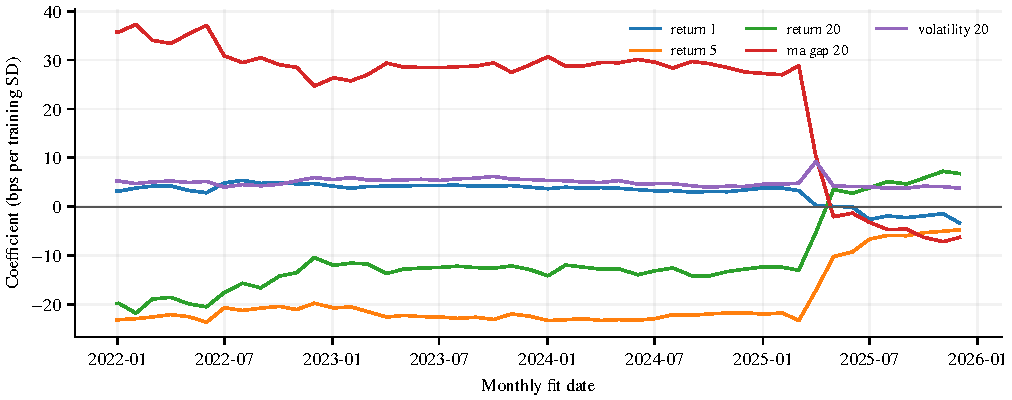
\includegraphics[width=.96\textwidth]{generated/coefficients.pdf}
 \caption{Coefficient paths on training-standardized inputs, in basis points per training SD. Signs and magnitudes are conditional associations among correlated features. The paths are not used to select features after testing.}
 \label{fig:coefappendix}
\end{figure}

\begin{table}[htbp]
 \centering\small
 \caption{Descriptive coefficient summary across the 49 fitted models. Sign changes count adjacent monthly estimates with different signs, not changes in the daily position.}
 \label{tab:coefsummary}
 \begin{tabular}{lrrrr}
\toprule
Feature & Mean (bps) & Min. (bps) & Max. (bps) & Sign changes \\
\midrule
\texttt{return\_1} & 2.918 & -3.353 & 5.376 & 1 \\
\texttt{return\_5} & -19.585 & -23.684 & -4.748 & 0 \\
\texttt{return\_20} & -10.991 & -21.827 & 7.227 & 1 \\
\texttt{ma\_gap\_20} & 23.807 & -7.187 & 37.297 & 1 \\
\texttt{volatility\_20} & 4.959 & 3.742 & 9.203 & 0 \\
\bottomrule
\end{tabular}

\end{table}

Coefficient changes can occur even with a stable data-generating relation because old observations leave the fixed-length window and new observations enter. Correlated predictors can redistribute weight among themselves. A large coefficient on the moving-average gap, for example, is not evidence that the corresponding univariate rule should replace the full model. The relation is estimated jointly, after scaling, and is assessed only through the frozen out-of-sample procedure. No coefficient-stability filter is added to improve the reported path.

\FloatBarrier
\section{Reproduction, Artifact Integrity, and Team Metadata}
\label{app:reproduction}
\subsection{Environment and exact stage commands}
Python 3.12 is the tested interpreter. Direct dependency versions are pinned in \code{requirements.txt}; a clean-install transitive environment is recorded in \code{requirements-lock.txt}. The seed is 42, while the Ridge SVD solve itself is deterministic for the stated inputs. Numerical libraries and platform-specific rendering can affect bytes, so input and result digests are reported separately from a claim of universal bitwise equality.

From a clean checkout, the recommended commands preserve published outputs and create a separate reproduction directory:
\begin{lstlisting}
python3.12 -m venv .venv
source .venv/bin/activate
python -m pip install -r requirements.txt
python -m pytest -q
python -m project2.pipeline all --workspace runs/reproduction
python -m project2.report --workspace runs/reproduction
\end{lstlisting}
The pipeline command downloads history only if its local cache is absent, checks data, builds features, evaluates four validation candidates, locks the selection, evaluates only the chosen holdout model, and writes tables and plots. The report command reads saved results, generates the paper's tables and vector figures, and compiles this LaTeX document. It does not fit a new trading model. Tectonic or a standard LaTeX installation is required for typesetting; that requirement is separate from Python packages.

Independent stage commands are available for inspection. A root-directory run is appropriate only when working with the published matching input snapshot, or when intentionally maintaining a separate documented experiment. Appending \code{--workspace runs/reproduction} to each pipeline stage uses the separate directory consistently.
\begin{lstlisting}
python -m project2.pipeline fetch
python -m project2.pipeline validate
python -m project2.pipeline test
python -m project2.pipeline figures
python -m project2.report
\end{lstlisting}

\subsection{Artifact map and preserved input identity}
\begin{table}[htbp]
 \centering\small
 \caption{Source-to-artifact map. Paths are repository-relative; no local absolute machine directories are required by the research pipeline.}
 \label{tab:artifacts}
 \begin{tabularx}{\textwidth}{@{}lX@{}}
 \toprule
 Artifact & Role \\
 \midrule
 \code{config.json} & Frozen research specification and separate, editable identity fields. \\
 \code{data/provenance.json} & Source options, retrieval metadata, observed coverage, and raw-file digest. \\
 \code{output/selection.json} & Selected penalty and protocol/input/validation fingerprints. \\
 \code{output/tables/test_predictions.csv} & Signals, holding dates, forecasts, outcomes, and positions. \\
 \code{output/tables/test_fit_audit.csv} & Eligible-window boundaries, means, scales, intercepts, and coefficients. \\
 \code{output/tables/test_path_*.csv} & Per-interval returns, fees, turnover, and compounded wealth. \\
 \code{output/run_manifest.json} & Original research environment, settings, sample dates, and result digests. \\
 \code{paper/main.tex} & Conference-style report source, with modular sections and bibliography. \\
 \code{paper/generated/} & Saved-result tables, vector figures, and source-artifact digests. \\
 \bottomrule
 \end{tabularx}
\end{table}

\begin{samepage}
The following SHA-256 identities distinguish the original input snapshot from the final prediction artifact:
\begin{center}
\begin{tabularx}{\textwidth}{@{}lX@{}}
\toprule
Artifact & SHA-256 \\
\midrule
Raw input & {\footnotesize\ttfamily\seqsplit{e59594912552818d0fce625e8c8f16efe49d88db067cd787c27995355aa46498}} \\
Predictions & {\footnotesize\ttfamily\seqsplit{0ccaeaf2351cf3c005bced9b61d1a2db97632c90aa4ba91c39a32692d81aaa2c}} \\
\bottomrule
\end{tabularx}
\end{center}
\end{samepage}
The raw price file is not redistributed. A fresh vendor download may change after history revisions or adjustment rounding. Exact result reproduction is conditional on a matching input snapshot; different input is a newly disclosed run. Within an established run, a changed protocol or raw-data digest causes the selection lock to refuse overwriting the original experiment.

\subsection{Integrity checks and clean-environment evidence}
The suite contains 11 tests covering: executable label alignment and dividend entitlement; future-price invariance of earlier features; common-factor adjustment invariance; mature-label eligibility; invariance of earlier forecasts and scaling to future changes; equality of recorded means with training-window means; monthly refit count; initial and terminal fees; cash and switching behavior; initial-capital drawdown; period-boundary allocation; and explicit failure on missing values and splits. Some tests cover multiple related cases. Synthetic fixtures exist only in this suite, never as a fallback for reported performance.

A clean-environment reproduction used a fresh isolated virtual environment and a fresh working directory with the same downloaded local input snapshot. The validation-grid, final-prediction, fit-audit, and headline-metric CSVs matched byte for byte. This verifies reproducibility conditional on that input; it is not a second independent market sample. The recorded evidence is in \code{output/reproducibility_check.json}. Hosted continuous integration checks the suite and rebuilds the report from published derived results without downloading changing market data.

The LaTeX tables and numeric macros are generated from the same frozen CSV/JSON results, and the typesetting build verifies that its source digests match those artifacts. Rewriting this report does not refit the trading strategy or alter the selected penalty. This separation matters because presentation improvements should not silently become a new model-selection exercise.

\subsection{Assumptions a reviewer should retain}
All results depend on next-open fills, a proportional pre-trade fee, zero cash interest, a zero Sharpe reference rate, and ex-date receivable crediting. There is no order-book depth or market impact model, no funding or borrow constraint because the strategy is unlevered and long-only, and no split event in the supported sample. Full-history adjusted-price ratios have the stated common-factor invariance but remain subject to arbitrary vendor corrections. The single-asset and four-year-holdout scope is narrow, and no formal superiority test or factor alpha is claimed.

\subsection{Team information and assistance disclosure}
Team identity and contribution fields are intentionally blank and excluded from the protocol digest; filling them does not change model selection. Before submission, add the actual group number, title-page roster, and genuine contributions, consistently with the Canvas group.

\begin{table}[htbp]
 \centering\small
 \caption{Team and contribution information, intentionally unfilled.}
 \begin{tabularx}{\textwidth}{@{}p{.26\textwidth}X@{}}
\toprule
Group / team name &  \\
Full member roster &  \\
\midrule
Member & Contribution \\
\midrule
\rule{0pt}{18pt} & \\
\rule{0pt}{18pt} & \\
\rule{0pt}{18pt} & \\
\rule{0pt}{18pt} & \\
\bottomrule
\end{tabularx}

\end{table}

Code and report drafting used AI assistance; all reported results come from the executed historical-data pipeline. The walkthrough uses disclosed synthetic narration over actual results and command outputs. Team members should review the artifacts, record true contributions, and follow course disclosure rules. No live trading is performed.
